%%%%%%%%%%%%%%%%%%%%%%%%%%%%%%%%%%%%%%%%%%%%%%%%%%%%%%%%%%%%%%%%%%%%%%%%%%%%%%%%
% Template for USENIX papers.
%
% History:
%
% - TEMPLATE for Usenix papers, specifically to meet requirements of
%   USENIX '05. originally a template for producing IEEE-format
%   articles using LaTeX. written by Matthew Ward, CS Department,
%   Worcester Polytechnic Institute. adapted by David Beazley for his
%   excellent SWIG paper in Proceedings, Tcl 96. turned into a
%   smartass generic template by De Clarke, with thanks to both the
%   above pioneers. Use at your own risk. Complaints to /dev/null.
%   Make it two column with no page numbering, default is 10 point.
%
% - Munged by Fred Douglis <douglis@research.att.com> 10/97 to
%   separate the .sty file from the LaTeX source template, so that
%   people can more easily include the .sty file into an existing
%   document. Also changed to more closely follow the style guidelines
%   as represented by the Word sample file.
%
% - Note that since 2010, USENIX does not require endnotes. If you
%   want foot of page notes, don't include the endnotes package in the
%   usepackage command, below.
% - This version uses the latex2e styles, not the very ancient 2.09
%   stuff.
%
% - Updated July 2018: Text block size changed from 6.5" to 7"
%
% - Updated Dec 2018 for ATC'19:
%
%   * Revised text to pass HotCRP's auto-formatting check, with
%     hotcrp.settings.submission_form.body_font_size=10pt, and
%     hotcrp.settings.submission_form.line_height=12pt
%
%   * Switched from \endnote-s to \footnote-s to match Usenix's policy.
%
%   * \section* => \begin{abstract} ... \end{abstract}
%
%   * Make template self-contained in terms of bibtex entires, to allow
%     this file to be compiled. (And changing refs style to 'plain'.)
%
%   * Make template self-contained in terms of figures, to
%     allow this file to be compiled.
%
%   * Added packages for hyperref, embedding fonts, and improving
%     appearance.
%
%   * Removed outdated text.
%
%%%%%%%%%%%%%%%%%%%%%%%%%%%%%%%%%%%%%%%%%%%%%%%%%%%%%%%%%%%%%%%%%%%%%%%%%%%%%%%%

\documentclass[letterpaper,twocolumn,10pt]{article}
\usepackage{usenix}

% to be able to draw some self-contained figs
\usepackage{tikz}
\usepackage{amsmath}
\usepackage{caption}

% inlined bib file
\usepackage{filecontents}

\usepackage{graphicx}
\graphicspath{ {./imgs/} }

%-------------------------------------------------------------------------------
\begin{filecontents}{\jobname.bib}
%-------------------------------------------------------------------------------
@InProceedings{hypsec,
  author =       {Li, Shih-Wei and Koh, John S. and Nieh, Jason},
  title =        {Protecting Cloud Virtual Machines from Commodity Hypervisor and Host Operating System Exploit},
  booktitle =    {Proceedings of the 28th USENIX Security Symposium},
  year =         2019,
  pages =        {1357--1374},
  note =         {\url{https://www.cs.columbia.edu/~nieh/pubs/security2019_hypsec.pdf}}
}
@InProceedings{sekvm,
  author =       {Li, Shih-Wei and Li, Xupeng and Gu, Ronghui and Nieh, Jason and Hui, John Z.},
  title =        {Formally Verified Memory Protection for a Commodity Multiprocessor Hypervisor},
  booktitle =    {Proceedings of the 30th USENIX Security Symposium.},
  year =         2021,
  pages =        {3953--3970},
  note =         {\url{https://www.usenix.org/system/files/sec21-li-shih-wei.pdf}}
}
@Misc{xuheng,
    author =        {Li, Xuheng},
    title =         {\text{Fall 23 Operating Systems 2 Homework}},
    year =          {2023},
    howpublished =  {\url{https://xuhengli.notion.site}},
    note =          {Accessed: 2023-12-21}
}
@Misc{arm,
    author =        {ARM Developer Documentation},
    title =         {Learn the architecture - AArch64 virtualization},
    howpublished =  {\url{https://developer.arm.com/documentation/102142/0100/Stage-2-translation}},
    note =          {Accessed: 2023-12-21}
}
@Misc{vmlinux.lds.S,
    author =        {XuhengLi (GitHub username)},
    title =         {vmlinux.lds.S in osdi23-paper114-sekvm},
    howpublished =  {\url{https://github.com/columbia/osdi23-paper114-sekvm/blob/ae/arch/arm64/kernel/vmlinux.lds.S}},
    note =          {Accessed: 2023-12-21}
}
@Misc{kernel-pgtable.h,
    author =        {XuhengLi (GitHub username)},
    title =         {kernel-pagetable.h in osdi23-paper114-sekvm},
    howpublished =  {\url{https://github.com/columbia/osdi23-paper114-sekvm/blob/ae/arch/arm64/include/asm/kernel-pgtable.h}},
    note =          {Accessed: 2023-12-21}
}
@Misc{el1.c,
    author =        {XuhengLi (GitHub username)},
    title =         {el1.c in osdi23-paper114-sekvm},
    howpublished =  {\url{https://github.com/columbia/osdi23-paper114-sekvm/blob/ae/arch/arm64/hypsec_proved/el1.c}},
    note =          {Accessed: 2023-12-21}
}
@Misc{kerneldocs,
    author =        {kernel.org},
    title =         {Chapter 6: Physical Page Allocation},
    howpublished =  {\url{https://www.kernel.org/doc/gorman/html/understand/understand009.html}},
    note =          {Accessed: 2023-12-22}
}
@Misc{page_alloc.c,
    author =        {Elixir Bootlin},
    title =         {page\_alloc.c in Linux v5.4.55},
    howpublished =  {\url{https://elixir.bootlin.com/linux/v5.4.55/source/mm/page_alloc.c#L4718}},
    note =          {Accessed: 2023-12-22}
}
@Misc{mmzone.h,
    author =        {Elixir Bootlin},
    title =         {mmzone.h in Linux v5.4.55},
    howpublished =  {\url{https://elixir.bootlin.com/linux/v5.4.55/source/include/linux/mmzone.h#L27}},
    note =          {Accessed: 2023-12-22}
}
@Misc{el2.c,
    author =        {XuhengLi (GitHub username)},
    title =         {el2.c in osdi23-paper114-sekvm},
    howpublished =  {\url{https://github.com/columbia/osdi23-paper114-sekvm/blob/ae/arch/arm64/hypsec_proved/el2.c}},
    note =          {Accessed: 2023-12-22}
}
@Misc{hypsec_host.h,
    author =        {XuhengLi (GitHub username)},
    title =         {hypsec\_host.h in osdi23-paper114-sekvm},
    howpublished =  {\url{https://github.com/columbia/osdi23-paper114-sekvm/blob/ae/arch/arm64/include/asm/hypsec_host.h}},
    note =          {Accessed: 2023-12-22}
}
\end{filecontents}

% %-------------------------------------------------------------------------------
\begin{document}
% %-------------------------------------------------------------------------------

%don't want date printed
\date{}

% make title bold and 14 pt font (Latex default is non-bold, 16 pt)
\title{\Large \bf FlexAlloc: Dynamic Memory Partitioning\\
    between the Corevisor and Hostvisor in SeKVM}

%for single author (just remove % characters)
\author{
{\rm Matthew Nelson}\\
Columbia University
\and
{\rm Ryan Wee}\\
Columbia University
\and
{\rm Zeheng Yang}\\
Columbia University
} % end author

\maketitle

%-------------------------------------------------------------------------------
\begin{abstract}
%-------------------------------------------------------------------------------
SeKVM is a hypervisor for ARM processors that protects the memory of guest
virtual machines (VMs) from an untrusted host machine. It comprises a
corevisor that runs at EL2, and a hostvisor that runs at EL1
to leverage the functionality of the untrusted host kernel. However, SeKVM
statically partitions memory between the corevisor and hostvisor at compile
time. This leads to memory wastage when the number of VMs is low, and an
inability to support the desired number of VMs when the number of VMs is high.
In this paper, we present FlexAlloc, an extension of SeKVM that allows dynamic
runtime partitioning of memory between the corevisor and the hostvisor. In
particular, the memory needed for the stage-2 page tables of a guest VM is
only allocated to the corevisor when a VM is created. This memory is then
returned to the hostvisor when a VM is destroyed. Existing implementions
of \textit{alloc\_pages} do not support allocating a contiguous region of memory
equal in size to the memory needed for a VM's stage-2 page tables. Hence,
FlexAlloc also modifies the iterators used to accesss a VM's stage-2 page
tables, so that the memory used for a VM's stage-2 page tables can be composed
of noncontiguous regions. Our work ensures that a machine running SeKVM uses
memory more efficiently, and also allows such machines to support a larger
number of guest VMs. This allows public cloud providers and organizations
running their own VMs to scale up their operations at a lower cost.
\end{abstract}

%-------------------------------------------------------------------------------
\section{Introduction and Background}
%-------------------------------------------------------------------------------

Virtual machines (VMs) have become increasingly popular over the past few
decades. In particular, they improve utilization of existing hardware by
allowing users to run multiple unmodified operating systems on a single machine.
A key concern when it comes to VMs is isolation. A single machine may be used to
run multiple VMs created by different users who generally want their data
to be protected from one another. As a result, hypervisors generally maintain
some sort of secure boundary between guest VMs. However, another important
aspect of isolation is protecting guest VMs from the host machine. A hypervisor
that fully trusts its host machine is vulnerable to malicious actors who
gain control of the host operating system itself. This is dangerous because
the host machine could be used to steal confidential corporate data or sensitive
personal information.

SeKVM is a formally verified hypervisor for ARM that isolates KVM's trusted computing
base into a small core~\cite{sekvm}. It builds on the previous work of HypSec,
which is a hypervisor that protects VMs from the host machine~\cite{hypsec}.
HypSec consists of two layers. The first layer is an untrusted
\textit{hostvisor}, which operates at EL1 together with the host operating
system. The hostvisor leverages many of the data structures and functions
built into the host operating system for VM management. The second layer is a
trusted \textit{corevisor}, which operates at the more privileged EL2 level.
This corevisor is responsible for isolating VMs from each other and from the
host machine. SeKVM builds on HypSec's design, with the main difference being
that its trusted computing base is formally verified. In SeKVM, the two layers
are termed \textit{KServ} and \textit{KCore} respectively. However, in this
paper, we use the terms hostvisor and corevisor to remain
consistent with the underlying HypSec kernel source code.

SeKVM protects guest VMs in three main areas: CPU, memory, and I/O. In the
area of memory, SeKVM leverages ARM hardware support for virtualization. ARM
allows hypervisors to control memory access using stage-2
translation~\cite{arm}. In particular, the guest operating systems and host
operating system each think they are using page tables to map a virtual address space to the
physical address space. However, in reality, they only control the mapping
of virtual addresses to intermediate physical addresses. When translating
virtual addresses, the MMU starts by using these page tables to translate
virtual addresses into intermediate physical addresses. However, it then
uses a second set of page tables to translate
intermediate phyiscal addresses into the actual machine physical addresses.
This second set of page tables, called stage-2 page tables, are controlled by
the hypervisor running at EL2. In the context of SeKVM, the stage-2 page tables
are managed by the corevisor. When the host operating system tries to
access some physical memory, the corevisor first checks that this
physical memory does not belong to a guest VM.

The hostvisor cannot be allowed to access the memory used to store
the stage-2 page tables of guest VMs. Otherwise, it could simply modify these
stage-2 page tables so that guest VMs write their data to memory that can be
accessed and manipulated by the hostvisor. In other words, the memory used for
these stage-2 page tables must `belong' to the corevisor. In SeKVM,
the corevisor is statically allocated this memory on bootup. This is done by
a linker script, which allocates some
contiguous region of memory for the stage-2 page tables and demarcates it using the labels \textit{stage2\_pgs\_start}
and \textit{stage2\_pgs\_end}~\cite{vmlinux.lds.S}. The size of this memory region is
determined by the macro \textit{STAGE2\_PAGES\_SIZE}~\cite{kernel-pgtable.h}. In
particular, this memory region is large enough to store the stage-2 page table
for the corevisor, the stage-2 page table for the hostvisor,
and the stage-2 page tables for sixteen guest VMs. The corevisor and hostvisor are
each allocated sixteen 2M pages for their stage-2 page tables, while each guest VM
is allocated four 2M pages. Altogether, the corevisor is given 96 2M
pages for all of these stage-2 page tables. During bootup, the hostvisor
allocates the beginning of this memory region to the corevisor and itself. It then
initializes the corevisor's VM-management data structure such that the remainder of this stage-2 page table memory region
is evenly divided between each of the sixteen possible guest VMs. In particular, the hostvisor sets
\textit{el2\_data->vm\_info[i].page\_pool\_start =
pool\_start + (STAGE2\_VM\_POOL\_SIZE * (i - 1))} for each possible VMID~\cite{el1.c}.
Here, \textit{vm\_info[i].page\_pool\_start} marks the start of the stage-2
page table for the \textit{i}th VM.

The key observation here is that this partitioning of memory is done statically
at compile time. In other words, the hostvisor cannot reclaim the memory it has
allocated to the corevisor. Similarly, the corevisor cannot ask for more memory
from the hostvisor. This is in contrast to the dynamic partitioning of memory
between the hostvisor and guest VMs. Guest VMs can request memory from the
hostvisor via a page fault, and the hostvisor can reclaim memory from guest VMs
using ballooning~\cite{hypsec}. The static partitioning of memory between the
hostvisor and the corevisor is undesirable for two reasons:

\begin{itemize}
    \item First, unused memory cannot be reclaimed from the corevisor. Say
    the number of VMs being run is $n$, such that $n < 16$. Then there will be
    $(16 - n) * 4$ 2M pages reserved for the stage-2 page tables of guest VMs that
    do not exist. Dynamic partitioning of memory would allow this memory to be reclaimed by the hostvisor, to
    alleviate memory pressure in the host. This memory could also be given to guest VMs, to
    alleviate memory pressure in these VMs. Giving VMs more memory would improve
    VM performance, because less data would need to be moved to the swap partition.
    \item Second, there is a hard upper limit on the number of VMs that can
    be supported by SeKVM. Users cannot add VMs above the limit of sixteen,
    because there will be no memory in the corevisor to support the stage-2
    page tables of these VMs. Users could always choose to statically allocate
    even more memory to the corevisor upon bootup, but this would exacerbate
    the problem of unused memory mentioned above.
\end{itemize}

Static allocation of memory to the corevisor is not limited to memory for the
stage-2 page tables of each VM. In addition to this, SeKVM also statically
allocates memory to the corevisor to store the metadata of each VM. The same linker script
mentioned above reserves another contiguous region of memory equal in size to 32
2M pages, and demarcates it using \textit{el2\_data\_start}
and \textit{el2\_data\_end}~\cite{vmlinux.lds.S}. This memory is given to the
corevisor on bootup. Part of this memory is used to
store an array of \textit{struct el2\_vm\_info} objects, where each object is
used to store the metadata of each guest VM. SeKVM could potentially also benefit
from dynamic allocation of the memory used to store this VM metadata, where
this memory is only given to the corevisor upon VM creation and returned to the
hostvisor upon VM deletion. However,
we choose not to focus on this because the size of each \textit{struct el2\_vm\_info} object
is 768 bytes. The total size of all of the \textit{struct el2\_vm\_info} objects
is 12288 bytes, which is less than four 4K pages in total. As a result, the
problem of unused memory is not as significant, since we waste at most four
4K pages of memory. In any case, memory can only be allocated at the
page granularity. Hence, in the case where we want to create a new VM and the new \textit{struct el2\_vm\_info} object
cannot be placed into the pages that have already been dynamically allocated to the corevisor, we will
inevitably end up having to allocate an entirely new 4K page. The majority of this new 4K page would then remain unused, until another VM is created. This
is not the case with VM stage-2 page tables, since the size of the stage-2 page
table for each VM is nicely page-aligned. With the \textit{struct el2\_vm\_info} objects, the problem of a hard upper limit
is also not as significant, since we could easily make the array larger without
incurring much memory overhead.

Although the metadata structs have a much smaller memory footprint than the stage-2 page tables,
we designed and partially implemented a fully generalized dynamic allocation interface that
could be used to support dynamic allocation for all metadata structs which we call the
Dynamic Page Manager (DPM). DPM handles all of the work required to receive and return
memory from the hostvisor allowing other "services" in EL2 to exchange memory with DPM using
a very similiar interface to the \textit{alloc\_pages} and \textit{free\_pages} interface available in EL1. We describe
this interface in detail in Section 4.

%-------------------------------------------------------------------------------
\section{Design and Implementation}
%-------------------------------------------------------------------------------

All of the source code described below can be found at \url{https://github.com/nelsonm2991/host-sekvm-project}.
Our implementation of FlexAlloc is based on SeKVM, which is in turn based on Linux v5.4.55.

\subsection{Modifying the page table iterators}

As described above, the original implementation of SeKVM statically
allocates sixteen contiguous 8M regions to the corevisor (Figure \ref{fig:sekvmvmregions}). When a VM is created,
the corevisor uses one of these contiguous 8M regions for the VM's stage-2
page table. To implement a system of dynamic allocation, we want the hostvisor
to dynamically reserve a contiguous 8M region at runtime when a VM is created, and then
pass this memory region to the corevisor. The kernel macro \textit{alloc\_pages}
is responsible for allocating a large number of contiguous physical pages~\cite{kerneldocs}.
Examining the implementation of this macro reveals that it eventually
calls \textit{\_\_alloc\_pages\_nodemask}, which checks that the order requested
is strictly less than \textit{MAX\_ORDER}~\cite{page_alloc.c}. \textit{MAX\_ORDER}
is in turn defined to be 11~\cite{mmzone.h}. This means that we cannot allocate
a contiguous region of memory larger than $2^{10} * 4K = 4M$. This
limit is set by the kernel because \textit{alloc\_pages} uses the buddy allocator,
which recursively splits available memory into half to find the best possible position for
a contiguous region of memory~\cite{kerneldocs}. However, this also makes it
undesirable to continuously allocate huge contiguous regions of memory.

\begin{figure}[h!tbp]
\centering
\captionsetup{justification=centering}
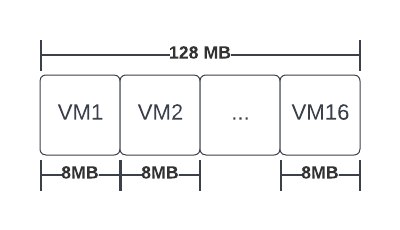
\includegraphics{sekvm_vm_region}
\caption{SeKVM: Layout of Statically-Allocated\\Region for VM Stage-2 Page Tables}
\label{fig:sekvmvmregions}
\end{figure}

\bigskip To get around this limitation, there are two possible approaches. The first approach
is to halve the size of the VM's stage-2 page table, so that it can fit within
a single contiguous 4M region of memory. Alternatively, we can fragment the VM's stage-2
page table such that it can be composed of multiple non-contiguous regions of memory, whose sizes in total add up to 8M. We
choose to implement the latter approach to avoid degrading VM performance, and to avoid
breaking the current implementation of the buddy allocator. In
particular, we fragment the VM's stage-2 page table so that it can be composed
of eight distinct 1M regions of memory. Each of these 1M regions must be contiguous,
but each region is distinct and need not be allocated contiguously with the
other 1M regions. As a result, the hostvisor can easily use \textit{alloc\_pages}
to allocate the memory needed for a guest VM's stage-2 page tables.

We implement this fragmentation by manipulating the iterators that provide the next useable
page at a given level. These iterators are used when traversing the stage-2 page table in order to record
an additional entry. In the original SeKVM implementation, the pages in each level of the stage-2 page table are
kept contiguous to one another, and never intermixed with pages from other levels.
Each iterator starts at a particular offset into the VM's statically allocated stage-2
page table region, and increments each time a new entry is consumed at that level. The design of these iterators means that they are limited to
only operating within a large, contiguous region. In particular, the PGD iterator operates over a \textit{16 * PAGE\_SIZE} region, the PUD
iterator operates over a \textit{SZ\_2M - (16 * PAGE\_SIZE)} region, and the PMD iterator operates over a \textit{3 * SZ\_2M} region.

In contrast, our design eliminates the need for all of these subregions to be contiguous to
one another and enables fragmentation within each subregion itself. Each iterator can be thought of as a page allocator specific to VM stage-2
page tables, and operates over a pool of eight, non-contiguous 1MB regions. The FlexAlloc iterators
first exhaust all pages from a given 1MB region. Once the current 1MB region is exhausted, FlexAlloc
will jump the iterators to the next 1MB region in the pool. Subsequent traversals of the
stage-2 page tables with the alloc flag enabled will pull pages from the seperate, second
non-contiguous 1M region. By removing the requirement for contiguous 8MB regions, FlexAlloc
enables reliable dynamic allocation of stage-2 page table regions.

We implement two versions of the FlexAlloc iterators. In the first version, we use a single,
generalized iterator shared across all levels of the stage-2 page table. In the SeKVM implementation,
the iterators are structured such that a PUD page will never be sandwiches between two PMD pages.
The first version of the FlexAlloc iterators ignores this semantic and instead is non-discriminatory
in regards to the particular level a page will be used in. However, we eventually decided to stop development of this
version before it was fully functional, in favor of version two which more closely resembles recent changes made to SeKVM's
stage-2 page table allocation scheme.

In the second implementation, we opt to enforce the semantic that pages at each specific level are
allocated from seperate pools, and thus never intermixed with one another. To accomplish this while still maintaining the same pool of non-contiguous 1MB regions,
we split the single, general iterator into nine distinct iterators. One iterator is used
for PUD pages, two iterators are used for PMD pages, and six iterators are used for PTE pages.
The number of iterators assigned to each level is based on the potential maximum number of
pages that could be consumed at that level, along with how many distinct 1MB regions each level
can be allocated from. When a page is allocated at a particular level, the correct iterator is chosen based on
its assigned level and whether or not its preceding iterators have been exhausted.

\begin{figure}[h!tbp]
\centering
\captionsetup{justification=centering}
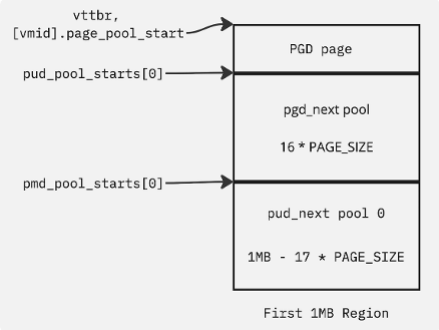
\includegraphics{firstmbregion}
\caption{FlexAlloc: Metadata Setup\\for First 1MB Region}
\label{fig:firstmbregion}
\end{figure}

\begin{figure}[h!tbp]
\centering
\captionsetup{justification=centering}
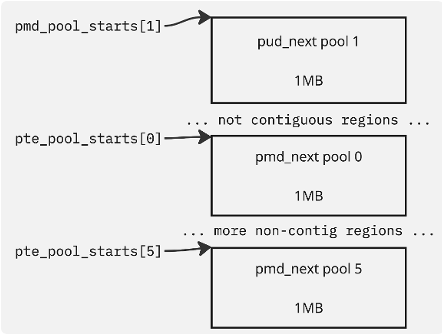
\includegraphics{otherregions}
\caption{FlexAlloc: Metadata Setup\\for Second to Eigth 1MB Regions}
\label{fig:otherregions}
\end{figure}

\bigskip Each level's iterators have a set number of regions from which to pull additional pages from. Lower
levels in the table have larger regions than higher levels in the table. When the current iterator
over a given region is exhausted, the iterator will jump to the next available region and pick up
where it left off.


\begin{verbatim}
static u64 inline get_pmd_next(u32 vmid) {
    ...
    // pool_index: available iterator
    // we are using
    pool_index =
      el2_data->vm_info[vmid].pte_pool_index;
    // pool_start: beginning of the region
    // the pool_index corresponds to
    pool_start =
      el2_data->vm_info[vmid].
      pte_pool_starts[pool_index];
    // used_pages: number of pages in this
    // region we have exhausted
    used_pages = el2_data->vm_info[vmid]
      .pte_used_pages_vm[pool_index];

    // If we've used up all the pages and we
    // have another region, then use the new
    // region.
    if (used_pages == PTE_ITER_MAX_PAGES &&
        pool_index + 1 <
        PTE_USED_ITER_COUNT) {
        pool_index += 1;
        el2_data->vm_info[vmid].
          pte_pool_index = pool_index;

        // Set the pool_start to the next
        // available PTE iterator.
        pool_start = el2_data->vm_info[vmid].
          pte_pool_starts[pool_index];
        used_pages = el2_data->vm_info[vmid].
          pte_used_pages_vm[pool_index];
    }

    // Make sure we have not exhausted all
    // pages across all regions.
    if (used_pages == PTE_ITER_MAX_PAGES &&
            pool_index ==
            PTE_USED_ITER_COUNT - 1) {
        __hyp_panic();
    }

    // Return the physical address of the
    // next page that this iterator can
    // allocate.
    return pool_start +
      (used_pages * PAGE_SIZE);
}
\end{verbatim}

The naming semantics of the iterators at each level can be confusing, so we feel it is worth
clarifying here. The PGD iterator allocates pages to use as entries inside of a PGD page. This
implies that the PGD iterator, as an example, actually allocates pages that are used in the
subsequent level, which in this case is the PUD. All iterators follow the pattern of allocating
pages for a given level to point to. These are actually pages in the next level
of the stage-2 page tables.

\subsection{Allocating memory to the corevisor}

FlexAlloc dynamically allocates eight 1M memory regions to the corevisor when a
VM is created. It does so by passing the base addresses of these eight 1M
regions as arguments to the \textit{HVC\_REGISTER\_KVM} hypercall. An alternative
implementation that we considered was creating a new \textit{HVC\_PASS\_MEM} hypercall to pass these
1M regions to the corevisor, and getting the hostvisor to call \textit{HVC\_PASS\_MEM}
before calling \textit{HVC\_REGISTER\_KVM}. However, we ultimately choose to
discard this alternative design because it leads to a more complicated
implementation. In particular, the corevisor would have to verify a one-to-one
correspondence between calls to \textit{HVC\_PASS\_MEM} and \textit{HVC\_REGISTER\_KVM}.
It would also have to handle malicious hostvisors that try to call
\textit{HVC\_REGISTER\_KVM} without calling \textit{HVC\_PASS\_MEM}. Morevoer,
adding an extra hypercall increases latency because it leads to more frequent
world-switches between the hostvisor running in EL1 and the corevisor running in EL2.

The \textit{HVC\_REGISTER\_KVM} hypercall eventually calls \textit{register\_kvm}
~\cite{el2.c}. Note that at this point we are in the corevisor, running at EL2.
Within this function, we preprocess the eight 1M regions to ensure that the
calls to \textit{alloc\_pages} in the hostvisor were successful, and to verify
that the memory regions provided actually belong to the hostvisor. We then set
the ownership of these memory regions to the corevisor, so that the host can
no longer access or manipulate the guest VM's stage-2 page tables. In particular,
we do the following:

\begin{verbatim}
for (i = 0; i < 8; ++i) {
    addr = page_starts[i];
    end = page_starts[i] + SZ_1M;

    /* ... */

    if (addr == 0) {
        // Hostvisor's alloc_pages() failed.
        __hyp_panic();
    }

    // Change the ownership of these pages
    // to the corevisor.
    do {
        index = get_s2_page_index(addr);
        owner = get_s2_page_vmid(index);

        if (owner != HOSTVISOR) {
            // The hostvisor shouldn't be
            // giving memory that belongs
            // to the corevisor or to a VM.
            __hyp_panic();
        }

        set_s2_page_vmid(index, COREVISOR);
        addr += PAGE_SIZE;
        ++page_cnt;
    } while (addr < end);
}
\end{verbatim}

\noindent We then build the VM's stage-2 page table using these eight 1M regions, by
populating the relevant fields in the \textit{struct el2\_data} object used
by the corevisor for VM management.

\subsection{Reclaiming memory from the corevisor}

When a VM is destroyed, FlexAlloc reclaims the eight 1M memory regions that were
previously allocated to the corevisor for the VM's stage-2 page table. Returning
this memory to the hostvisor ensures that it does not remain unused in corevisor
memory. Unlike the case of VM creation, there is no hypercall made directly to
the corevisor when a VM is destroyed. Hence, we create a new \textit{HVC\_DESTROY\_KVM}
hypercall that mirrors the \textit{HVC\_REGISTER\_KVM} hypercall used during VM
creation. In particular, on ARM architectures, if the \textit{CONFIG\_VERIFIED\_KVM} macro is defined,
we call \textit{hypsec\_arch\_destroy\_vm}. This function in turn calls \textit{hypsec\_destroy\_kvm},
which ultimately invokes the \textit{HVC\_REGISTER\_KVM} hypercall with the corresponding
VMID. We do not pass the base addresses of the eight 1M memory regions as arguments
to this hypercall, since the corevisor can access them directly by reading the
relevant fields of the \textit{struct el2\_data} object. Once we are in the
corevisor running in EL2, we return the eight memory regions to the hostvisor.
We then return to the hostvisor running in EL1, which can then call \textit{\_\_free\_pages}
on each of the eight 1M regions.

%-------------------------------------------------------------------------------
\section{Evaluation}
%-------------------------------------------------------------------------------

We evaluate FlexAlloc by running it on a QEMU-emulated Raspberry Pi 4. In
particular, we run VMWare Fusion Professional Version 13.0.0 on a 2018 x86-64 Macbook
Pro running MacOS Ventura 13.6.1. Using VMWare, we create a VM
with 4 processor cores and 12 GB memory running Ubuntu 22.04.3 LTS. On this
VM, we run QEMU 6.2.0 to emulate a Raspberry Pi 4. This emulated Raspberry
Pi 4 serves as our host machine, on which we run an SeKVM with the FlexAlloc
extension. Our guest VMs run vanilla Linux v5.4.

Using FlexAlloc, we boot up a guest VM and verify that it is able to start up
without any kernel panics. We use \textit{print\_string} to verify that we
are passing eight distinct 1M regions to the corevisor when the VM is created.
We test a case where the 1M regions are not contiguous, and verify that our
modified page table iterators are able to successfully handle a VM stage-2 page
table that is non-contiguous. We also shut down the guest VM and verify that
all eight 1M regions are returned to the hostvisor. We compare the base address
of each region allocated during VM creation against the base address of each
region reclaimed during VM shutdown, and verify that they match each other.

In order to make sure that the host can reasonably be expected to find 8x 1MB
contiguous regions when booting a VM, we evaluated how many successful
\textit{alloc\_pages(1MB)} calls could be made before failure. To reproduce our tests,
simply compile host-sekvm-project with the \textit{ALLOC\_STRESS\_TEST} macro defined.
Across our three trails, after booting host SeKVM with the FlexAlloc extension,
we were able to achieve between 7049 and 7054 successful 1MB allocations
from \textit{alloc\_pages(1MB)} calls. Since each VM only needs 8 successful allocations,
we believe that the upperbound on the number of VM's due to potential \textit{alloc\_pages(1MB)}
failures is sufficiently high.

We verified the changes in corevisor's memory footprint by checking the number of
pages owned by the corevisor according to the \textit{s2\_pages} array in \textit{el2\_data} at key points
throughout the VM boot and destruction processes. On a host running SeKVM without the
FlexAlloc extension, we observed that the Corevisor owned 65549 pages before booting a VM,
while running a VM, and after destroying a VM. On a host running SeKVM with the FlexAlloc
extension, we observed that the Corevisor owned 32768 pages before VM boot, 34817 pages
during the life of the VM, and 32768 pages after destroying the VM. Note that FlexAlloc also
reduces the static stage2\_region size in the linker script to zero as it is no longer needed.
These findings show that FlexAlloc is able to successfully receive, use, and handback pages
given by the host for usage exclusively as VM stage-2 page tables.

%-------------------------------------------------------------------------------
\section{Shortcomings and Future Work}
%-------------------------------------------------------------------------------

\subsection{Shortcomings in design}

One key shortcoming of FlexAlloc is that it is not formally verified. In
this sense, FlexAlloc is less like SeKVM and more like HypSec. It provides isolation guarantees
in principle, but cannot be logically proven to be secure. In particular, there
are a few major flaws in FlexAlloc when it comes to isolating guest VMs from
the host machine. For instance, the current implementation of FlexAlloc
does not use \textit{memset} to zero out the memory given to it by the hostvisor
for the VM's stage-2 page table. This presents a danger if the MMU tries to
read from a page table entry that should not actually exist, but that has
previously been written into the memory region by the hostvisor. We also occasionally
observed stalls when booting subsequent VMs after shutting down other VMs that we
believe were caused by failing to \textit{memset} the pages to zero. For example, the second
VM to boot after booting and shutting down the first VM can receive pages with non-zero data
that, when interpretted as page table entries, lead to undefined behavior.

Another flaw is that
FlexAlloc does not verify that the eight 1M regions are actually distinct and
do not overlap with one another. Hence, FlexAlloc still fundamentally relies on
a non-malicious hostvisor, and would require further patches to be fully secure.
To fix this, FlexAlloc can simply have an added check that verifies all of the
physical addresses received from the host are unique, 1MB aligned, and non-overlapping.

Another key shortcoming of our design is that it does not fully implement
dynamic memory partitioning between the corevisor and hostvisor outside of stage-2 page tables for VMs. As mentioned in
the introduction, another area in which corevisor memory scales with the number
of VMs is in maintaining \textit{struct el2\_vm\_info} objects that record the
metadata associated with each guest VM. Currently, we still statically allocate
a fixed-size array of \textit{struct el2\_vm\_info} objects in corevisor
memory ~\cite{hypsec_host.h}. This essentially preserves the hard cap on the
number of guest VMs that can be run. An easy fix would be to keep this array
as a statically-allocated array, while increasing the number of elements. Since each
\textit{struct el2\_vm\_info} object is only 768 bytes, this would not waste a
significant amount of memory even if fewer than sixteen VMs are created. Regarding the
\textit{shared\_data\_region}, since each VM requires a \textit{struct kvm}, the size of
this region would either need to be dynamically allocated or the static size would
need to be increases in order to lift the 16 VM cap present in SeKVM. However, since the static region
size has been decreased by 128 MB within FlexAlloc and the size of \textit{struct kvm}'s is relatively
small, inflating this region to accomodate 32+ VMs would still result in substantial memory savings
thanks to FlexAlloc's changes. In the Future Work section, we propose a potential solution to
the issue of bringing dynamic allocation to EL2 metadata structures that are not page aligned
which we call DPM.


\subsection{Shortcomings in evaluation}

We also do not fully evaluate our implementation. For one, we do not stress-test our implementation by running a large number
of VMs. To do this, we would have to modify the macros used to define the current
sixteen-VM limit. It is entirely conceivable that the hostvisor might not be able
to allocate 1M contiguous regions of memory past a certain point if memory
pressure and external fragmentation are high. In this case, the hostvisor would
not be able to allocate the memory regions needed for the corevisor to create
the stage-2 page table for a new VM. We could perhaps delay this limit by breaking
the VM stage-2 page tables down into even smaller regions of memory. In addition, we do not verify whether fragmenting the stage-2 page table results
in any degradation in VM performance. Given the less-than-ideal test environment
we have at our disposal, we did not investigate performance metrics related to execution time
for our implementation and only considered memory footprint metrics. Ideally, we would run a memory-intensive
benchmark on our guest VMs to verify that our iterators work properly under a
high memory load across multiple VMs.

\subsection{Future work}

A possible area of future work is exploring other allocators designed for
allocating large chunks of contiguous memory. We fragment the VM stage-2 page tables
into eight distinct 1M pages, because \textit{alloc\_pages} does not allow us
to allocate contiguous regions larger than 4M. We also wanted to be reasonably certain
that the size of our regions would not impeed the host's ability to launch VMs. It might be possile to avoid this
by looking at other Linux memory allocators explicitly designed for the purpose
of large contiguous allocations and adding such an allocator to the host.

\subsection{Dynamic Page Manager}
To enable dynamic allocation of EL2 memory in general beyond just the scope of
a VM's stage-2 page tables, we also designed but did not fully implement
a dynamic page manager (DPM). DPM is a system that exposes an interface for other ``services'' within EL2 to
utilize dynamic allocation for their memory regions, while hiding the implementation of actually receiving memory from
and returning memory to the host. This would be another interesting area of future work.

%-------------------------------------------------------------------------------
\section{Conclusions}
%-------------------------------------------------------------------------------

We have designed and implemented FlexAlloc, a system for dynamic memory
partitioning between the corevisor and hostvisor in SeKVM. In particular, we
modify SeKVM so that the hostvisor allocates memory to the corevisor when a VM is
created, and reclaims memory from the corevisor when a VM is destroyed. As a
result, the memory for a VM's stage-2 page table does not need to be statically
allocated to the corevisor upon bootup. This system reduces the wastage of memory
when VM demand is low, and increases the number of VMs that can be run
on a single machine when VM demand is high. We also make a distinct contribution in terms of fragmenting
a VM's stage-2 page table so that it can be composed of multiple noncontiguous
regions of memory, instead of a single contiguous 8M region. Altogether, this
system improves hardware utilization and reduces VM operating costs.

%-------------------------------------------------------------------------------
\section*{Acknowledgments}
%-------------------------------------------------------------------------------

Shih-Wei Li, John S. Koh, and Jason Nieh implemented HypSec, which serves as
the predecessor to SeKVM. Shih-Wei Li, Xupeng Li, Ronghui Gu, Jason Nieh, and
John Zhuang Hui implemented and formally verified SeKVM. Xuheng Li wrote a
helpful set of notes describing the boot and initialization process in SeKVM,
as well as the steps needed to build and run SeKVM~\cite{xuheng}. Jason Nieh and
Xuheng Li provided helpful comments on the project and helped with the design
of FlexAlloc. This paper was written as part of the class COMS E6118 Operating
Systems II at Columbia University.

%-------------------------------------------------------------------------------
\bibliographystyle{plain}
\bibliography{\jobname}

%%%%%%%%%%%%%%%%%%%%%%%%%%%%%%%%%%%%%%%%%%%%%%%%%%%%%%%%%%%%%%%%%%%%%%%%%%%%%%%%
\end{document}
%%%%%%%%%%%%%%%%%%%%%%%%%%%%%%%%%%%%%%%%%%%%%%%%%%%%%%%%%%%%%%%%%%%%%%%%%%%%%%%%

%%  LocalWords:  endnotes includegraphics fread ptr nobj noindent
%%  LocalWords:  pdflatex acks

%-------------------------------------------------------------------------------
% \section{Floating Figures and Lists}
% \label{sec:figs}
%-------------------------------------------------------------------------------

%---------------------------
% \begin{figure}
% \begin{center}
% \begin{tikzpicture}
%   \draw[thin,gray!40] (-2,-2) grid (2,2);
%   \draw[<->] (-2,0)--(2,0) node[right]{$x$};
%   \draw[<->] (0,-2)--(0,2) node[above]{$y$};
%   \draw[line width=2pt,blue,-stealth](0,0)--(1,1)
%         node[anchor=south west]{$\boldsymbol{u}$};
%   \draw[line width=2pt,red,-stealth](0,0)--(-1,-1)
%         node[anchor=north east]{$\boldsymbol{-u}$};
% \end{tikzpicture}
% \end{center}
% \caption{\label{fig:vectors} Text size inside figure should be as big as
%   caption's text. Text size inside figure should be as big as
%   caption's text. Text size inside figure should be as big as
%   caption's text. Text size inside figure should be as big as
%   caption's text. Text size inside figure should be as big as
%   caption's text. }
% \end{figure}
%% %---------------------------


% Here's a typical reference to a floating figure:
% Figure~\ref{fig:vectors}. Floats should usually be placed where latex
% wants then. Figure\ref{fig:vectors} is centered, and has a caption
% that instructs you to make sure that the size of the text within the
% figures that you use is as big as (or bigger than) the size of the
% text in the caption of the figures. Please do. Really.

% In our case, we've explicitly drawn the figure inlined in latex, to
% allow this tex file to cleanly compile. But usually, your figures will
% reside in some file.pdf, and you'd include them in your document
% with, say, \textbackslash{}includegraphics.

% Lists are sometimes quite handy. If you want to itemize things, feel
% free:

% \begin{description}

% \item[fread] a function that reads from a \texttt{stream} into the
%   array \texttt{ptr} at most \texttt{nobj} objects of size
%   \texttt{size}, returning returns the number of objects read.

% \item[Fred] a person's name, e.g., there once was a dude named Fred
%   who separated usenix.sty from this file to allow for easy
%   inclusion.
% \end{description}
